\documentclass{beamer}

\usepackage{tikz}
\usepackage{amsfonts}
\usepackage{soul}
\usepackage{fontawesome}

\usetikzlibrary{decorations.pathreplacing}
\usetikzlibrary{fit}
\usetikzlibrary{calc}
\usetikzlibrary{positioning}
\usetikzlibrary{arrows.meta}
\usetikzlibrary{shapes}

%\setbeamertemplate{navigation symbols}{%
%\insertslidenavigationsymbol \insertframenavigationsymbol \insertsubsectionnavigationsymbol \insertsectionnavigationsymbol \insertdocnavigationsymbol \insertbackfindforwardnavigationsymbol \hspace{1em}%
%\usebeamerfont{footline} \insertframenumber/\inserttotalframenumber%
%}

\beamertemplatenavigationsymbolsempty
\addtobeamertemplate{navigation symbols}{}{%
    %\usebeamerfont{footline}%
    \footnotesize
    \usebeamercolor[fg]{footline}%
    \hspace{1em}%
    \insertframenumber/\inserttotalframenumber
}

\usetheme{Frankfurt}

\title{Using stigmergy as a computational memory in the design of recurrent neural networks}
\author{Federico A. Galatolo}
\date{20 February 2019}

\begin{document}

\maketitle

\section{Introduction}
\begin{frame}
    \frametitle{Time-Series Static Classification}
    \begin{columns}
        \begin{column}{0.2\textwidth}
            \begin{itemize}
                \item MLP
                \item CNN
                \item ...
            \end{itemize}
        \end{column}
        \begin{column}{0.8\textwidth}
            \newcommand{\myblock}[4]{
    \node (#4) at (#1, #2) [draw, minimum width=1cm, minimum height=1cm] {\small  #3};
}

\newcommand{\mybrace}[3]{
    \draw [decorate,decoration={brace,amplitude=10pt,mirror,raise=4pt},yshift=0pt]
    ($(#1, #2) + (-0.5,-0.4)$) -- ++(3, 0) node (#3) [black,midway,xshift=0.8cm] {};
}

\def\xrow{6}
\def\yrow{0}

\begin{center}
    \begin{tikzpicture}
        \foreach \x/\xtext/\name in {0/$X_0$/x0, 1/$X_1$/x1, 2/$X_2$/x2, 3/$X_3$/x3, 4/{...}/x4, 5/$X_{n-2}$/x5, 6/$X_{n-1}$/x6}{
            \myblock{\x}{\xrow}{\xtext}{\name};
        }

        \node (center) at (3,3) [draw, minimum width=3cm, minimum height=2cm] {Static System};
        
        \foreach \x/\xtext/\name in {1.5/$Y_0$/y0, 2.5/$Y_1$/y1, 3.5/{...}/y2, 4.5/$Y_{n-1}$/y3}{
            \myblock{\x}{\yrow}{\xtext}{\name};
        }

        \uncover<2>{
            \mybrace{0}{6}{b1}
            \draw [->] ($(b1) + (-0.8,-0.5)$) -- (center.north);
            \draw [->] (center.south) -- (y0.north);
        }

       \uncover<3>{
            \mybrace{1}{6}{b2}
            \draw [->] ($(b2) + (-0.8,-0.5)$) -- (center.north);
            \draw [->] (center.south) -- (y1.north);
        }

        \uncover<4>{
            \mybrace{4}{6}{b3}
            \draw [->] ($(b3) + (-0.8,-0.5)$) -- (center.north);
            \draw [->] (center.south) -- (y3.north);
        }

    \end{tikzpicture}
\end{center}
        \end{column}
    \end{columns}
\end{frame}

\begin{frame}
    \frametitle{Time-Series Static Classification}
    \begin{itemize}
        \item[\checkmark] You can use any existing ML Architecture
        \item[$\times$] Window size choice
        \item[$\times$] Long-lived relationships are impossible to infer 
    \end{itemize} 
\end{frame}


\begin{frame}
    \frametitle{Time-Series Dynamic Classification}
    \begin{columns}
        \begin{column}{0.2\textwidth}
            \begin{itemize}
                \item RNN
                \item LSTM
                \item ...
            \end{itemize}
        \end{column}
        \begin{column}{0.8\textwidth}
            \newcommand{\myblock}[4]{
    \node (#4) at (#1, #2) [draw, minimum width=1cm, minimum height=1cm] {\small  #3};
}

\def\xrow{6}
\def\yrow{0}

\begin{center}
    \begin{tikzpicture}
        \foreach \x/\xtext/\name in {0/$X_0$/x0, 1/$X_1$/x1, 2/$X_2$/x2, 3/$X_3$/x3, 4/{...}/x4, 5/$X_{n-2}$/x5, 6/$X_{n-1}$/x6}{
            \myblock{\x}{\xrow}{\xtext}{\name};
        }

        \node (center) at (3,3) [draw, minimum width=3cm, minimum height=2cm] {Dynamic System};
        
        \foreach \x/\xtext/\name in {1.5/$Y_0$/y0, 2.5/$Y_1$/y1, 3.5/{...}/y2, 4.5/$Y_{n-1}$/y3}{
            \myblock{\x}{\yrow}{\xtext}{\name};
        }

        \uncover<2>{
            \draw [->] (x0.south) -- (center.north);
            \draw [->] (center.south) -- (y0.north);
            \node at ($(center.south) + (0,0.3cm)$) [draw, minimum height=0.6cm, minimum width=1cm] {$S_0$};
        }

       \uncover<3>{
            \draw [->] (x1.south) -- (center.north);
            \draw [->] (center.south) -- (y1.north);
            \node at ($(center.south) + (0,0.3cm)$) [draw, minimum height=0.6cm, minimum width=1cm] {$S_1$};
        
        }

        \uncover<4>{
            \draw [->] (x6.south) -- (center.north);
            \draw [->] (center.south) -- (y3.north);
            \node at ($(center.south) + (0,0.3cm)$) [draw, minimum height=0.6cm, minimum width=1cm] {$S_{n-1}$};
        }

    \end{tikzpicture}
\end{center}
        \end{column}
    \end{columns}
\end{frame}

\begin{frame}
    \frametitle{Time-Series Dynamic Classification}
    \begin{itemize}
        \item[\checkmark] The system knows the concept of time
        \item[\checkmark] Can autonomously decide what to remember and forget
        \item[$\times$] Ad-Hoc solutions
        \item[$\times$] Highly engineered
    \end{itemize}
\end{frame}

\begin{frame}
    \frametitle{RNN $\ne$ LSTM}
    \vspace{0.3cm}
    \begin{itemize}
        \item RNN and LSTM are often used as synonyms in literature 
        \item Has been proven that ``Vanilla recursion'' performs poorly  
        \item LSTM are the state of the art for Time Series Classification 
    \end{itemize}
    \def\dist{0.35}

\begin{center}
    \begin{tikzpicture}
        \node (system) at (0,3) [draw, minimum height=4cm, text width=3cm,align=center] {Feed Forward Architecture};
        
        \draw [->, thick] (-5,3) -- (system);
        \draw [->, thick] (system) -- (5, 3);


        \pause
        
        \path [draw, ->, thick] ($(system.east) + (0, -\dist)$) |- ($(system.east) + (\dist, -\dist)$) 
        |- ($(system.south east) + (\dist, -\dist)$) |- ($(system.south west) + (-\dist, -\dist)$)
        |- ($(system.west) + (-\dist, -\dist)$) |- ($(system.west) + (0, -\dist)$)  ;

        \uncover<3>{
            \node (rnn) at (0,3) [draw, dashed, minimum height=5.25cm, text width=5cm, label={Recurrent Architecture}] {};
        }

    \end{tikzpicture}
\end{center}
\end{frame}

\begin{frame}
    \frametitle{A deep look inside an LSTM cell}
    \newcommand{\empt}[2]{$#1^{\langle #2 \rangle}$}

\begin{center}
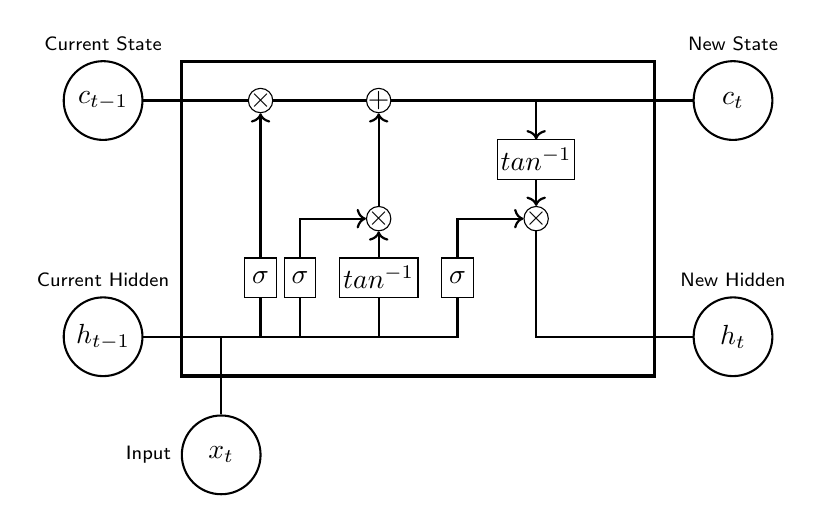
\begin{tikzpicture}[
    cell/.style={
        rectangle, 
        draw,
        very thick,
        },
    operator/.style={
        circle,
        draw,
        inner sep=-0.5pt,
        minimum height =.2cm,
        },
    function/.style={
        ellipse,
        draw,
        inner sep=1pt
        },
    ct/.style={
        circle,
        draw,
        line width = .75pt,
        minimum width=1cm,
        inner sep=1pt,
        },
    gt/.style={
        rectangle,
        draw,
        minimum width=4mm,
        minimum height=5mm,
        inner sep=1pt
        },
    mylabel/.style={
        font=\scriptsize\sffamily
        },
    ArrowC1/.style={
        thick,
        },
    ArrowC2/.style={
        thick,
        },
    ]

    \node [cell, minimum height =4cm, minimum width=6cm] at (0,0){} ;

    \node [gt] (ibox1) at (-2,-0.75) {$\sigma$};
    \node [gt] (ibox2) at (-1.5,-0.75) {$\sigma$};
    \node [gt, minimum width=1cm] (ibox3) at (-0.5,-0.75) {$tan^{-1}$};
    \node [gt] (ibox4) at (0.5,-0.75) {$\sigma$};

    \node [operator] (mux1) at (-2,1.5) {$\times$};
    \node [operator] (add1) at (-0.5,1.5) {+};
    \node [operator] (mux2) at (-0.5,0) {$\times$};
    \node [operator] (mux3) at (1.5,0) {$\times$};
    \node [gt] (func1) at (1.5,0.75) {$tan^{-1}$};

    \node[ct, label={[mylabel]Current State}] (c) at (-4,1.5) {$c_{t-1}$};
    \node[ct, label={[mylabel]Current Hidden}] (h) at (-4,-1.5) {$h_{t-1}$};
    \node[ct, label={[mylabel]left:Input}] (x) at (-2.5,-3) {$x_t$};

    \node[ct, label={[mylabel]New State}] (c2) at (4,1.5) {$c_t$};
    \node[ct, label={[mylabel]New Hidden}] (h2) at (4,-1.5) {$h_t$};
 
    \draw [ArrowC1] (c) -- (mux1) -- (add1) -- (c2);

    \draw [ArrowC2] (h) -| (ibox4);
    \draw [ArrowC1] (h -| ibox1)++(-0.5,0) -| (ibox1); 
    \draw [ArrowC1] (h -| ibox2)++(-0.5,0) -| (ibox2);
    \draw [ArrowC1] (h -| ibox3)++(-0.5,0) -| (ibox3);
    \draw [ArrowC1] (x) -- (x |- h)-| (ibox3);

    \draw [->, ArrowC2] (ibox1) -- (mux1);
    \draw [->, ArrowC2] (ibox2) |- (mux2);
    \draw [->, ArrowC2] (ibox3) -- (mux2);
    \draw [->, ArrowC2] (ibox4) |- (mux3);
    \draw [->, ArrowC2] (mux2) -- (add1);
    \draw [->, ArrowC1] (add1 -| func1)++(-0.5,0) -| (func1);
    \draw [->, ArrowC2] (func1) -- (mux3);

    \draw [-, ArrowC2] (mux3) |- (h2);

\end{tikzpicture}
\end{center} \pause
    \begin{columns}
        \begin{column}{0.5\textwidth}
            \begin{itemize}
                \item $f_t = \sigma(W_f x_t + U_f h_t + b_f)$ \pause
                \item $i_t = \sigma(W_i x_t + U_i h_t + b_i)$ \pause
            \end{itemize}
        \end{column}
        \begin{column}{0.5\textwidth}
            \begin{itemize}
                \item $i_c = tan^{-1}(W_c x_t + U_c h_t + b_c)$ \pause
                \item $c_t = f_t \circ c_{t-1}$ \pause + $i_t \circ i_c$
            \end{itemize}
        \end{column}
    \end{columns}
\end{frame}

\begin{frame}
    \frametitle{A deep look inside an LSTM cell}
    \begin{itemize}
        \item $f_i = \sigma (W_f x_i + U_f h_{i-1} + b_f)$
        \item $i_i = \sigma (W_i x_i + U_i h_{i-1} + b_i)$
        \item $o_i = \sigma (W_o x_i + U_o h_{i-1} + b_o)$
        \item $c_i = \sigma (f_i \circ c_{i-1} + i_i \circ tan^{-1}(W_c X_i + U_c h_{i-1} + b_c))$
        \item $h_t = o_i * tan^{-1}(c_i)$
    \end{itemize}
    \vspace{0.5cm}
    Using
    \begin{itemize}
        \item $W_f,\;W_i,\;W_o,\;W_C \in R^{n\times h}$
        \item $U_f,\;U_i,\;U_o,\;U_c \in R^{h\times h}$
        \item $b_f,\;b_i,\;b_o,\;b_c \in R^h$
    \end{itemize}
    \vspace{0.5cm}

    \pause

    \begin{center}
        \Large Can we do better?
    \end{center}
    
    \pause

    \begin{center}
        \Large Can we do \textbf{simpler}?
    \end{center}
\end{frame}

\section{Stigmergic Memory}
\begin{frame}
    \frametitle{Let's take a step back}
    \pause
    \begin{columns}
        \begin{column}{0.5\textwidth}
            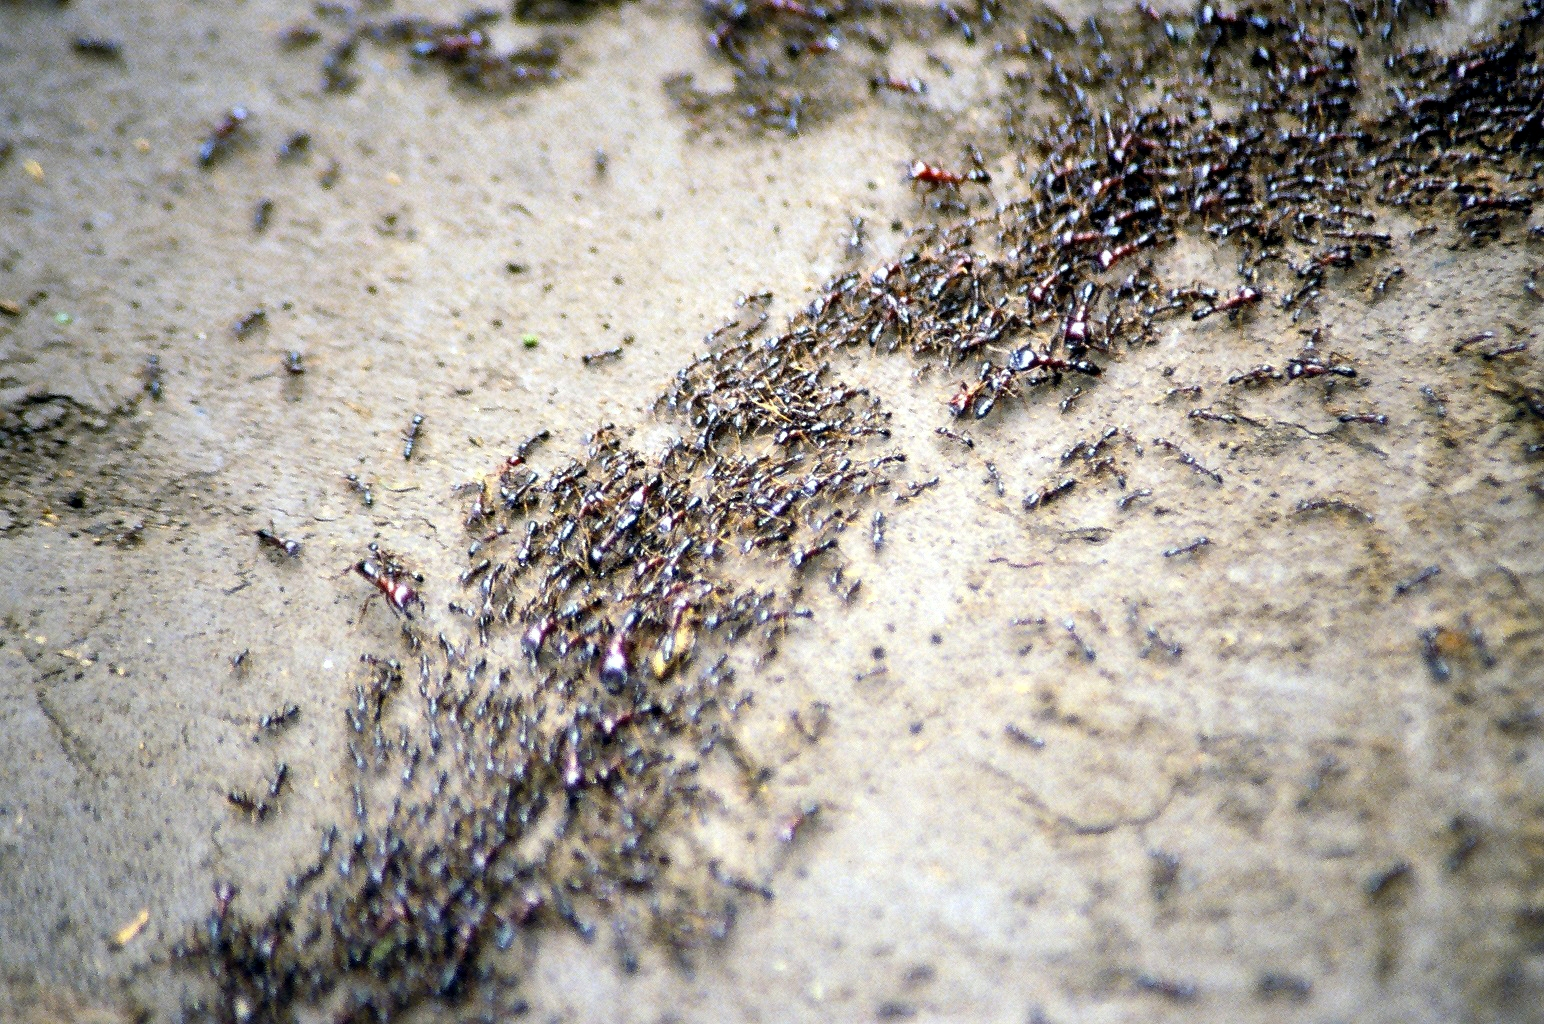
\includegraphics[width=\textwidth]{img/ants.jpg}
        \end{column}
        \pause
        \begin{column}{0.5\textwidth}
            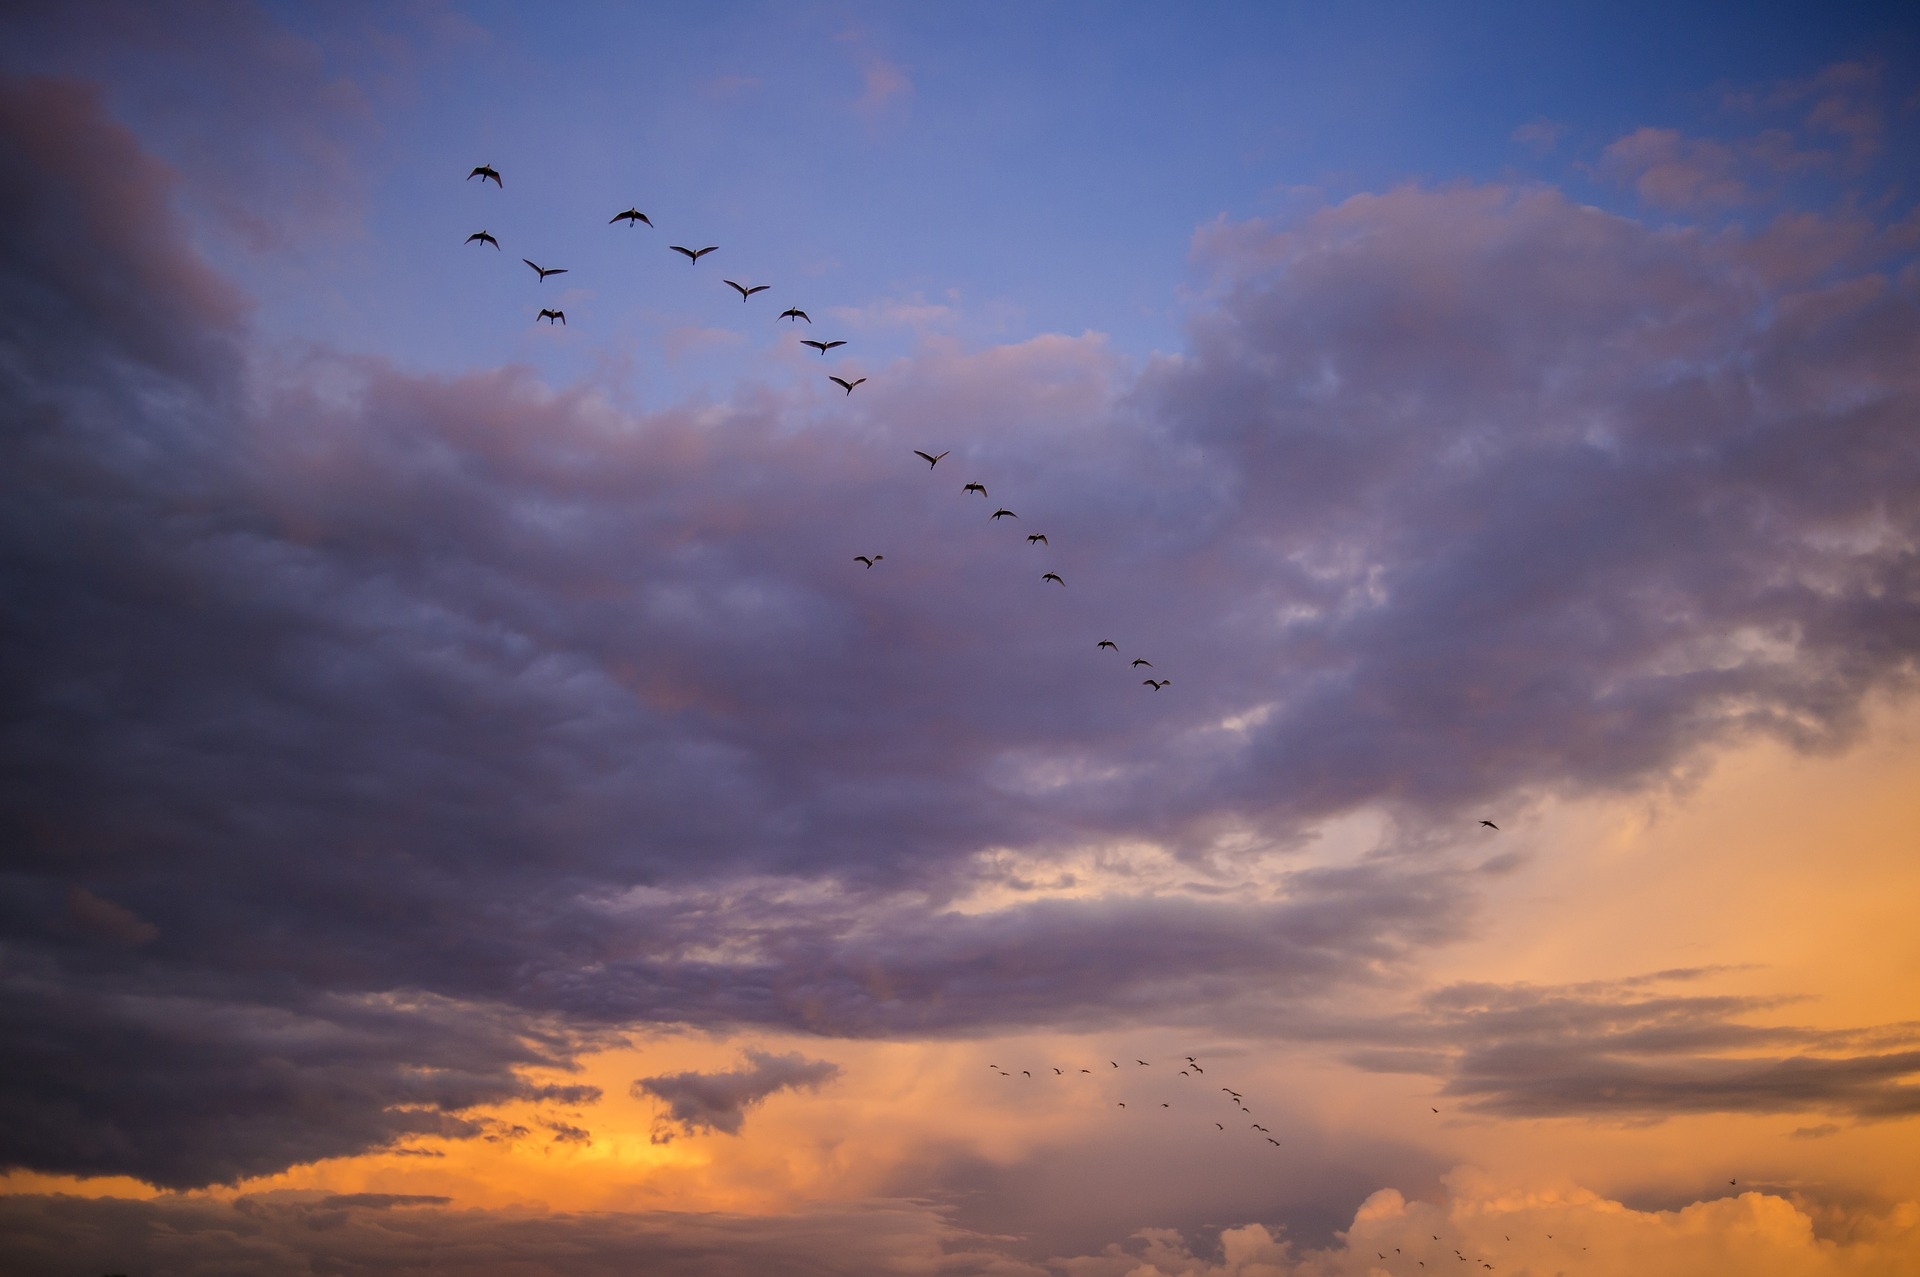
\includegraphics[width=\textwidth]{img/birds.jpg}
        \end{column}
        \pause
    \end{columns}
    \vspace{0.5cm}
    \begin{itemize}
        \item Complex behaviors can \textbf{emerge} from simple ones
        \item Emergence is a key phenomenon in nature
        \item \textbf{Stigmergy} is one of the tools nature uses to achieve emergence
    \end{itemize}
    \vspace{0.3cm}
    \pause
    \begin{center}
        Can we \textbf{emerge} a computational memory using the \textbf{stigmergy}?
    \end{center}
\end{frame}

\begin{frame}
    \frametitle{Biological Stigmergy}
    \begin{center}
        Implemented in nature via pheromonic marks 
    \end{center}
    \pause
    \def\hoffset{0.2}
\def\voffset{0.5}

\begin{center}
    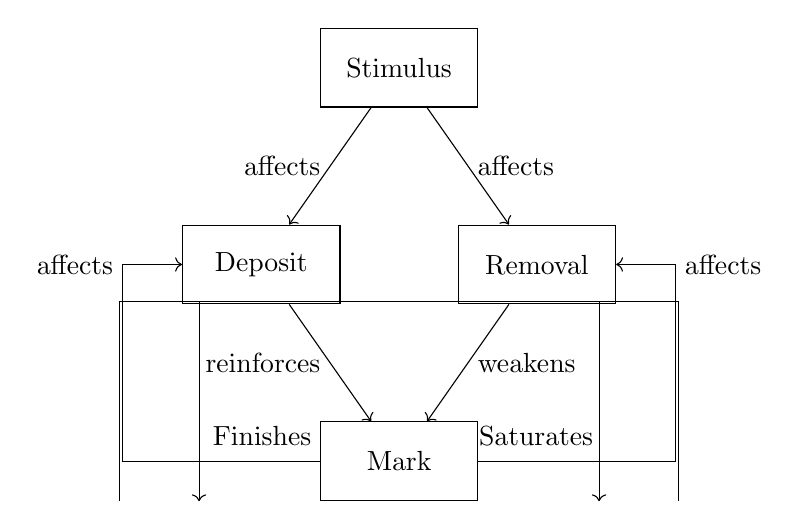
\begin{tikzpicture}[
            cell/.style={
                rectangle, 
                draw,
                minimum width=2cm,
                minimum height=1cm
            }
        ]
        \node (mark) at (2.5,0) [cell] {Mark};
        
        \pause
        
        \node (stimulus) at (2.5,5) [cell] {Stimulus};
        
        \pause
        
        \node (deposit) at (0.75,2.5) [cell] {Deposit};
        \node (removal) at (4.25,2.5) [cell] {Removal};
        
        \pause

        \draw [->] (stimulus) -- (deposit) node[midway,left] {affects};
        \draw [->] (stimulus) -- (removal) node[midway,right] {affects};

        \pause
        
        \draw [->] (deposit) -- (mark) node[midway, left] {reinforces};
        
        \pause
        
        \draw [->] (removal) -- (mark) node[midway, right] {weakens};

        \pause

        \draw [->] (mark.west) |- ($(mark.west) + (-2.5,.0)$) |- (deposit.west) node[midway, left] {affects};
        \draw [->] (mark.east) |- ($(mark.east) + (2.5,.0)$)  |- (removal.east) node[midway, right] {affects};        
        
        \pause

        \draw [->] ($(mark.south east) + (-\hoffset,0) $) |- ++(0, -\voffset) |- ($(mark.south) + (\hoffset,-\voffset)$) -- ++(0, \voffset) node [midway, below, xshift=0.8cm, yshift=-0.2cm] {Finishes};
        \draw [->] ($(mark.south west) + (\hoffset,0) $) |- ++(0, -\voffset) |- ($(mark.south) + (-\hoffset,-\voffset)$) -- ++(0, \voffset) node [midway, below, xshift=-0.8cm, yshift=-0.2cm] {Saturates};

    \end{tikzpicture}
\end{center}
\end{frame}

\begin{frame}
    \frametitle{Computational Stigmergy}
    \begin{center}
    \begin{tikzpicture}[
            cell/.style={
                rectangle, 
                draw,
                minimum width=2cm,
                minimum height=1cm
            },
            operator/.style={
                circle,
                draw,
                inner sep=-0.5pt,
                minimum height =.5cm,
            }
        ]
        \node (deposit) at (0,2.5) [cell] {Deposit};
        \node (removal) at (0,-2.5) [cell] {Removal};

        \pause

        \node (plus) [operator] at (0,0) {+};
        \draw [->] (deposit) -- (plus) node[midway, right] {+};
        \draw [->] (removal) -- (plus) node[midway, right] {-};
        
        \pause

        \node (clamp) at (1.5,0) [operator] {C};
        \draw [->] (plus) -- (clamp);
        \draw [->] (clamp.east) |- ++(0.5,0) |- ++(0, -0.75) |- ($(plus.west) + (-0.5,-0.75)$) |- ++(0, 0.75) |- (plus.west) ;

        \pause

        \node (memory) at (0,0) [draw, dashed, minimum height=3cm, minimum width=6cm] {};
        \draw [->] (clamp.east) -- ++(2.5,0);


    \end{tikzpicture}
\end{center}
\end{frame}

\begin{frame}
    \frametitle{Stigmergic Memory ML Architecture}
    \def\hoffset{0.5}
\def\voffset{0.3}

\begin{center}
    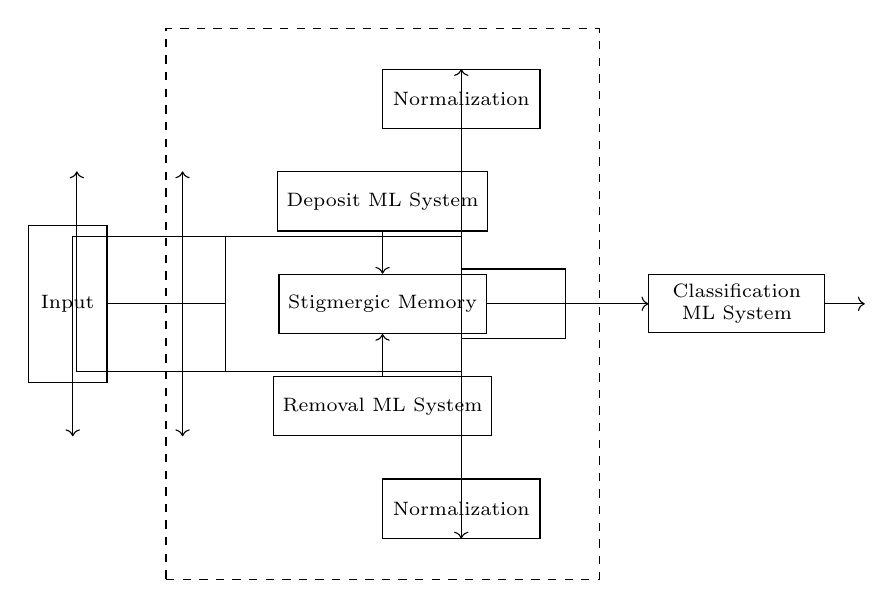
\begin{tikzpicture}[
            vertical/.style={
                rectangle, 
                draw,
                minimum width=1cm,
                minimum height=2cm,
            },
            horizontal/.style={
                rectangle, 
                draw,
                minimum width=2cm,
                minimum height=0.75cm
            }
        ]
        \tikzstyle{every node}=[font=\scriptsize]
        
        \pause

        \node (input) at (1,0) [vertical] {Input};
        
        \pause

        \node (space) at (5,0) [horizontal] {Stigmergic Memory};

        \pause

        \node (mark) at (5,1.3) [horizontal] {Deposit ML System};
        \node (tick) at (5,-1.3) [horizontal] {Removal ML System};

        \pause

        \draw [->] (input.east) |- ++(1.5,0) |- ($(mark.north west) + (\hoffset,\voffset)$) -- ++(0, -\voffset);
        \draw [->] (input.east) |- ++(1.5,0) |- ($(tick.south west) + (\hoffset,-\voffset)$) -- ++(0, \voffset);
        \draw [->] (mark) -- (space);
        \draw [->] (tick) -- (space);
        
        \pause

        \node (l1) at (6,2.6) [horizontal] {Normalization};
        \node (l2) at (6,-2.6) [horizontal] {Normalization};

        \pause

        \draw [->] (space.east) |- ++(1,0) |- ($(l1.north) + (1,\voffset)$) |- ($(l1.north) + (0,\voffset)$) -- (l1.north);
        \draw [->] (space.east) |- ++(1,0) |- ($(l2.south) + (1,-\voffset)$) |- ($(l2.south) + (0,-\voffset)$) -- (l2.south);
        \draw [->] (l1.south) |- ($(mark.north) + (\hoffset,\voffset)$) -- ++(0,-\voffset);
        \draw [->] (l2.north) |- ($(tick.south) + (\hoffset,-\voffset)$) -- ++(0,\voffset);

        \pause

        \node (wrapper) at (space) [draw, dashed, rectangle, minimum height=7cm, minimum width=5.5cm] {};
        \node (class) at (9.5,0) [draw, rectangle, text width=2cm, align=center] {Classification ML System};
        \draw [->] (space.east) -- (class);
        \draw [->] (class.east) -- ++(0.5, 0);


    \end{tikzpicture}
\end{center}
\end{frame}


\section{Experiments}
\begin{frame}
    \frametitle{Experimental Stigmergic ML Systems}
    Neural Networks Used as Deposit, Removal and Classification Systems
    \vspace{1.5cm}
    \begin{center}
    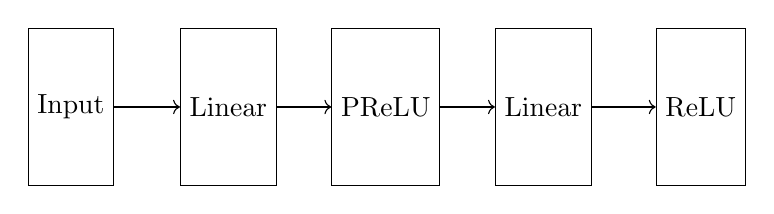
\begin{tikzpicture}[
        vertical/.style={
            rectangle, 
            draw,
            minimum width=1cm,
            minimum height=2cm,
        }
    ]

    \node (input) at (0,0) [vertical] {Input};
    \node (l1) at (2,0) [vertical] {Linear};
    \node (p1) at (4,0) [vertical] {PReLU};
    \node (l2) at (6,0) [vertical] {Linear};
    \node (p2) at (8,0) [vertical] {ReLU};

    \draw [->] (input) -- (l1);
    \draw [->] (l1) -- (p1);
    \draw [->] (p1) -- (l2);
    \draw [->] (l2) -- (p2);
    

    \end{tikzpicture}
\end{center}
\end{frame}

\begin{frame}
    \frametitle{Experimental Architectures}
    \begin{itemize}
        \item Stigmergic Memory NNs
        \item LSTMs
        \item Vanilla RNNs
        \item FF NNs (only with spatial dataset)
    \end{itemize}
\end{frame}

\begin{frame}
    \frametitle{Experimental Results: Spatial MNIST}
    \newcommand{\pararrow}[1]{
    \draw [->, thick] (-2,#1) -- (-0.5,#1);
}

\begin{center}
    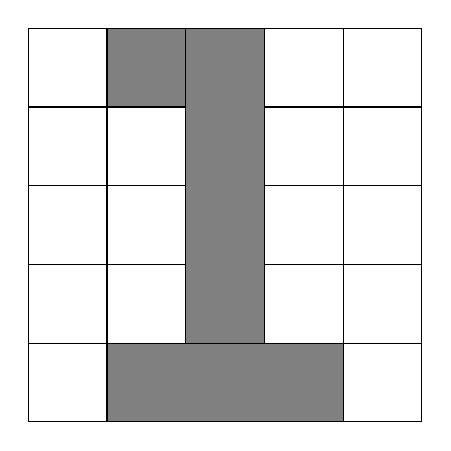
\begin{tikzpicture}
        \draw [step=1,black,thin] (0,0) grid (5,5);

        \draw [fill=gray] (2,0) rectangle (3,5);
        \draw [fill=gray] (1,0) rectangle (4,1);
        \draw [fill=gray] (1,4) rectangle (2,5);

        \uncover<2>{
            \pararrow{4.5}
        }
        \uncover<3>{
            \pararrow{3.5}
        }
        \uncover<4>{
            \pararrow{2.5}
        }
        \uncover<5>{
            \pararrow{1.5}
        }
        \uncover<6>{
            \pararrow{0.5}
        }

    \end{tikzpicture}
\end{center}
\end{frame}

\begin{frame}
    \frametitle{Experimental Results: Spatial MNIST}
    \begin{table}
        \begin{tabular}{l | c | c}
            Architecture & N. Parameters & Accuracy \\
            \hline
            \text{Stigmergic Memory} & 3190 & $96.5 \pm 0.5$ \% \\
            Static Feed Forward & 328810 & $95.1 \pm 0.02$ \% \\
            LSTM & 3360 & $94.3 \pm 0.1$ \% \\
            RNN & 3482 & $76.6 \pm 0.3$ \% \\
        \end{tabular}
    \end{table}
    \vspace{0.5cm}
    \begin{itemize}
        \item Outperforms LSTMs, Vanilla RNNs and FFs
        \item Best performances, smaller number of parameters
    \end{itemize}
\end{frame}

\begin{frame}
    \frametitle{Experimental Results: Temporal MNIST}
    
\begin{center}
    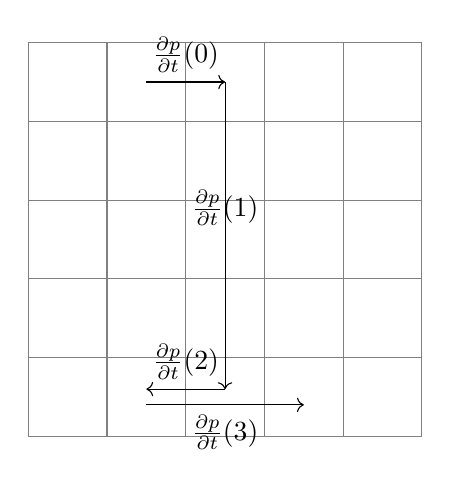
\begin{tikzpicture}
        \draw [step=1,gray,thin] (0,0) grid (5,5);

        \pause
        \draw [->] (1.5, 4.5) -- (2.5, 4.5) node[midway, above] {$\frac{\partial p}{\partial t}(0)$};

        \pause
        \draw [->] (2.5, 4.5) -- (2.5, 0.6) node[midway, above] {$\frac{\partial p}{\partial t}(1)$};

        \pause
        \draw [->] (2.5, 0.6) -- (1.5, 0.6) node[midway, above] {$\frac{\partial p}{\partial t}(2)$};

        \pause
        \draw [->] (1.5, 0.4) -- (3.5, 0.4) node[midway, below] {$\frac{\partial p}{\partial t}(3)$};


    \end{tikzpicture}
\end{center}
\end{frame}

\begin{frame}
    \frametitle{Experimental Results: Temporal MNIST}
    \begin{table}
        \begin{tabular}{l | c | c}
            Architecture & N. Parameters & Accuracy \\
            \hline
            LSTM & 5490 & $94.96 \pm 0.2$ \% \\
            \textbf{Stigmergic Memory} & 5420 & $94.67 \pm 0.7$ \% \\
            RNN & 5480 & $72.95 \pm 11$ \% \\
        \end{tabular}
    \end{table}
    \vspace{0.5cm}
    \begin{itemize}
        \item Outperforms Vanilla RNNs
        \item Same performances as LSTMs
    \end{itemize}
\end{frame}

\begin{frame}
    \frametitle{Keep in touch}
    \begin{center}
        \large You can find the pytorch implementation on GitHub
        
\includegraphics[width=.30\textwidth]{img/qr.png} \\
        \small https://github.com/galatolofederico/icpram2019
    \end{center}
    \begin{columns}
        \begin{column}{.5\textwidth}
            \begin{itemize}
                \item [\faEnvelope] federico.galatolo@ing.unipi.it
                \item [\faPaperPlane] @galatolo
            \end{itemize}
        \end{column}
        \begin{column}{.5\textwidth}
            \begin{itemize}
                \item [\faGlobe] federico.galatolo@ing.unipi.it
                \item [\faGithub] @galatolofederico
            \end{itemize}
        \end{column}
    \end{columns}
\end{frame}


\end{document}



